\begin{frame}{Third Milestone's achievements}
%\begin{variableblock}{What's done?}{bg=cyan,fg=white}{bg=white,fg=black}
%{



\begin{itemize}
	
	\item[\textcolor{green}
	{\Checkmark}] 100 \% open source
	
	\item[\textcolor{green}
	{\Checkmark}] GUI for user interaction
	
	\item[\textcolor{green}
	{\Checkmark}] Fairness functional to control Peters' scheme smoothness
	
		\item[\textcolor{green}
	{\Checkmark}] Conversion back to CAD
	
	\item[\textcolor{green}
	{\Checkmark}] Boolean operation support
	
	\item[\textcolor{green}
	{\Checkmark}] Test Cases
	
	\item[\textcolor{green}{\Checkmark}] Fully integrated pipeline 


\end{itemize}

\end{frame}

\begin{frame}{Outlook \& future work}
\begin{itemize}
\item Increase robustness of surface reconstruction \\
{\footnotesize \textcolor{blue}{Big amount of work: include topology checks and guarantee correct ambiguity treatment}}
\item Improve parameter estimation
\begin{itemize}
\item[--] complexity of algorithm \\ {\footnotesize \textcolor{blue}{current implementation has $\mathcal{O}\left(n^2\right)$ complexity}}
\item[--] accuracy of result \\ {\footnotesize \textcolor{blue}{not always projection onto the correct patches}}
\end{itemize}
\item Determine approximation error for our algorithm
\begin{itemize}
\item[--] Topology checks\\ {\footnotesize \textcolor{blue}{see above}}
\item[--] Accuracy estimates\\ {\footnotesize \textcolor{blue}{accuracy metrics? Important for estimation of reliability of results and basis for adaptivity}}
\end{itemize}
\item Develop a fully adaptive scheme \\ {\footnotesize \textcolor{blue}{Big amount of work: important for big patches and resolution of relatively small features, see testcase GE Bracket}}
\item Exchange ToPy with a faster solution \\ {\footnotesize \textcolor{blue}{Important because ToPy is currently bottleneck, faster solution is available}}
\end{itemize}
\end{frame}
\begin{frame}{Further remarks \& Discussion}
\begin{itemize}
\item \textcolor{blue}{isogeometric analysis as an completely different approach for the whole problems (anyhow there are many open questions)}
\item \textcolor{blue}{isogeometric analysis for shape optimization after topology optimization?}
\end{itemize}
\end{frame}


\begin{frame}{Results}
\begin{figure}
%\vspace{-.7cm}	
%\hspace{-2cm}
		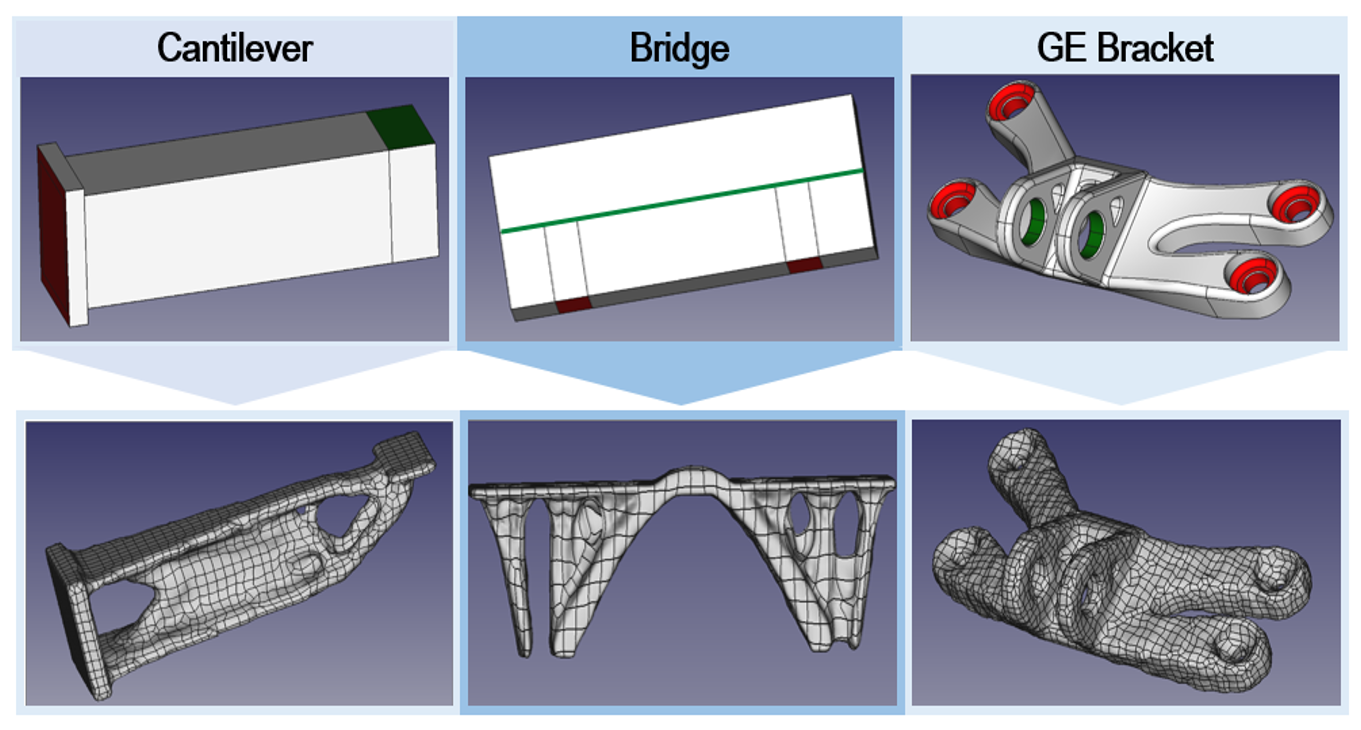
\includegraphics[width=1\linewidth]{Pictures/SecondHalf/TestCases.png}
		\end{figure}
GE Bracket design already optimized\textsuperscript{4} and only reconstructed.
\end{frame}
\begin{frame}
\begin{figure}

\vspace{-.7cm}	
\hspace{-2cm}		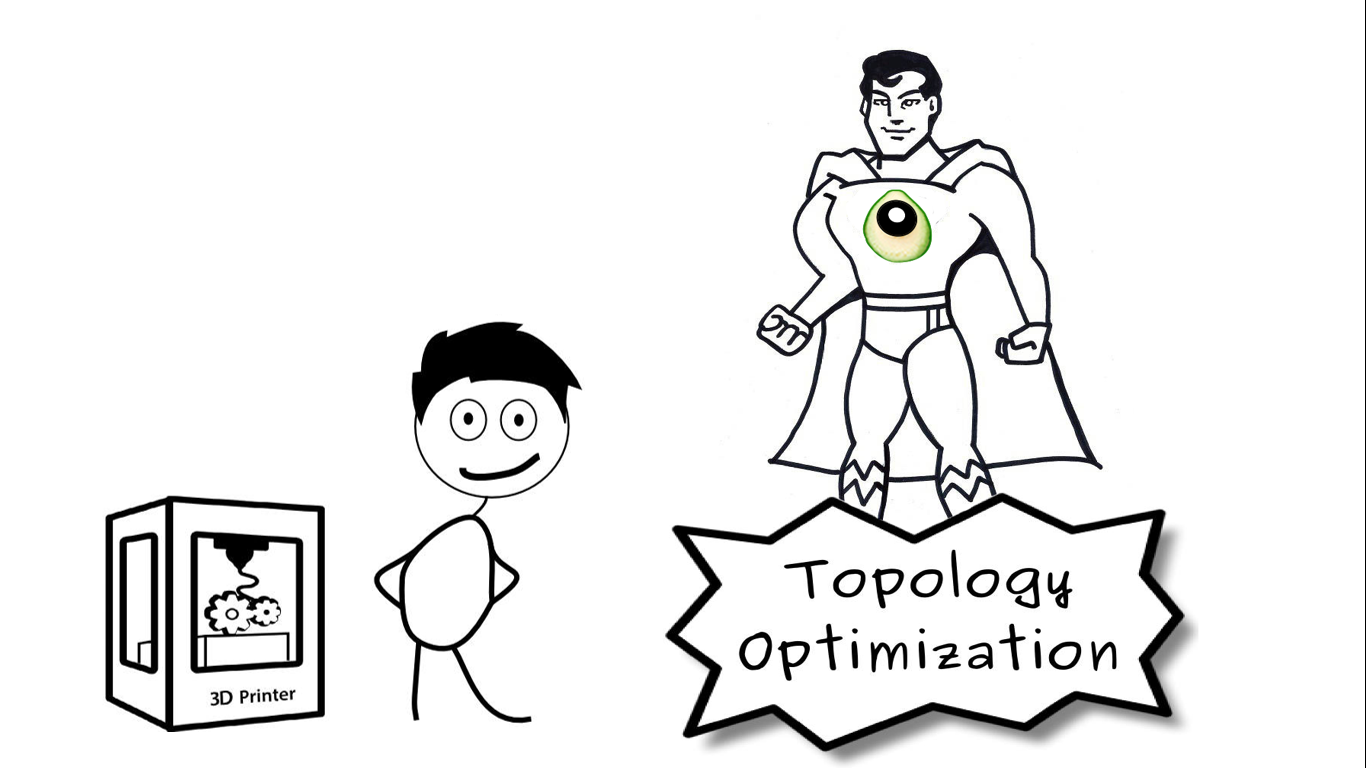
\includegraphics[width=1.2\linewidth]{Pictures/animations/animation_10.png}
		\end{figure}

\end{frame}





%%%%%%%%%%%%%%%%%%%%%%%%%%%%%%%%%%%%%%%
%%%OLD SLIDES

%\begin{frame}{What is next?}
%\begin{variableblock}{What's done?}{bg=cyan,fg=white}{bg=white,fg=black}
%{
%\begin{itemize}

%\item<+-> Topology Optimization
%\begin{itemize}
%	\item[\textcolor{green}{\Checkmark}] Pipeline from CAD model to optimized voxel model
%	\item[\textcolor{green}{\Checkmark}] User input of boundary conditions
%	\item[\textcolor{black}{\VarClock}] Support for complex geometries
%	\item[\textcolor{red}{\XSolidBrush}] GUI for user interaction
%\end{itemize}

%\item<+-> Surface Extraction
%\begin{itemize}
%	\item[\textcolor{green}{\Checkmark}] Dual Contouring for simple geometries
%	\item[\textcolor{green}{\Checkmark}] Provide necessary data for Surface Fitting
%	\item[\textcolor{black}{\VarClock}] Interfaces
	%\item[\textcolor{red}{\XSolidBrush}] Adaptive and topology safe Dual Contouring
%\end{itemize}

%\item<+-> Surface Fitting
%\begin{itemize}
	%\item[\textcolor{green}{\Checkmark}] B--spline fitting using least squares
	%\item[\textcolor{green}{\Checkmark}] Smooth connection of patches using Peters' scheme
	%\item[\textcolor{red}{\XSolidBrush}] Conversion back to CAD
%\end{itemize}
%\end{itemize}
%}
%\end{variableblock}
%\end{frame}
















